% sudo apt-get install texlive-latex-base
% sudo apt-get install texlive-fonts-extra
% sudo apt-get install texlive-latex-recommended
% sudo apt-get install texlive-lang-cyrillic

%------------------------------------------------------------------------------

\documentclass[11pt]{beamer}
\usetheme{Boadilla}
\usefonttheme{professionalfonts}
\usefonttheme[onlylarge]{structurebold}
\setbeamertemplate{navigation symbols}{}

%------------------------------------------------------------------------------

\usepackage[utf8]{inputenc} % возможность использования Unicode-символов в исходных файлах

\usepackage{amsmath} % для поддержки расширенных математических символов
\usepackage{amsfonts} % для поддержки математических шрифтов
\usepackage{amssymb} % для поддержки расширенных математических символов
\usepackage{graphicx} % для поддержки рисунков

\usepackage[english,russian]{babel} % поддержка переносов слов

%------------------------------------------------------------------------------

\title[]{Общий подход к классификации и ранжированию документов при неточных сравнительных оценках}
\author[И.Ю.~Ботян, Л.В.~Уткин]{И.Ю.~Ботян\andЛ.В.~Уткин}
\institute[СПбГЛТУ]{\large Санкт-Петербургский государственный лесотехнический университет}
\date[SCM-2014]{\large SCM-2014, Санкт-Петербург, 21-23 мая 2014}

%------------------------------------------------------------------------------

\DeclareGraphicsExtensions{.png}

\newcommand{\Rho}{%
	\mathcal{P}%
}

%------------------------------------------------------------------------------

\begin{document}

\graphicspath{ {./img/} }

%------------------------------------------------------------------------------
\begin{frame}

\titlepage

\end{frame}
%------------------------------------------------------------------------------
\begin{frame}{Введение. Задача классификации}

\begin{itemize}
	\begin{center}
		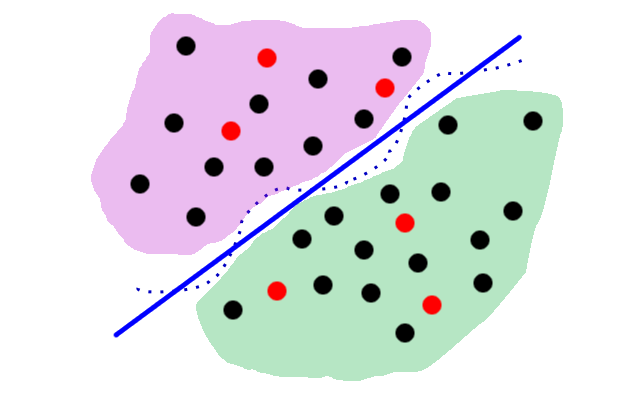
\includegraphics[scale=0.35]{classification}
	\end{center}
\end{itemize}

\end{frame}
%------------------------------------------------------------------------------
\begin{frame}{Традиционные и интервальные оценки экспертов}

\begin{itemize}
	\item \textbf{Пример:} результаты запроса в поисковой системе
	\item Одиночные экспертные оценки (простые)
		\begin{center}
			
\includegraphics[scale=0.4]{simple_judgment}
		\end{center}
	\item Групповые экспертные оценки (интервальные)
		\begin{center}
			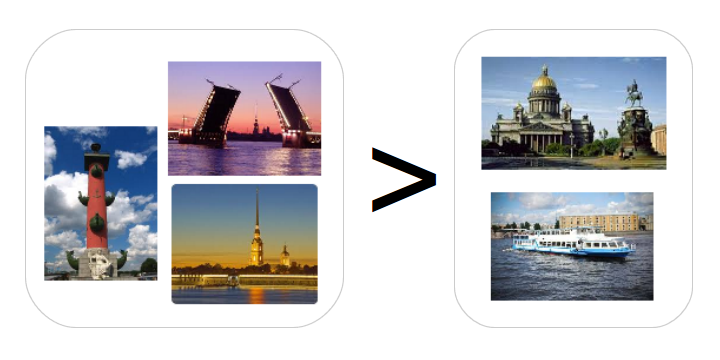
\includegraphics[scale=0.4]{interval_judgment}
		\end{center}
	\item \underline{Не существует} подходов на основе интервальных оценок
\end{itemize}

\end{frame}
%------------------------------------------------------------------------------
\begin{frame}{Стандартная постановка задачи классификации}

\begin{center}
		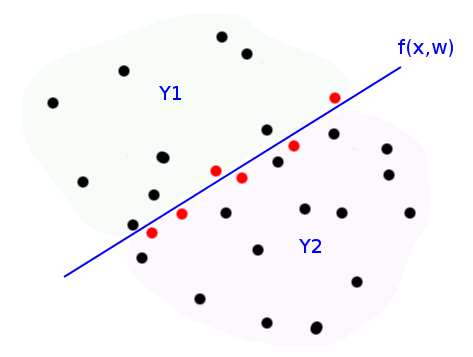
\includegraphics[scale=0.3]{standard_classification_problem}
	\end{center}

\begin{itemize}
	\item Параметры \(\mathbf{w}\) находятся путём вычисления функционала риска
		\[R(\mathbf{w}) = \int \limits_{\chi \times \{-1, +1\}} L(f, \mathbf{x}, y) \mathrm{d} F_0(\mathbf{x}, y).\]
	\item \(L(f, \mathbf{x}, y)\) - функция потерь \\
		\(0\) - классификация верна, иначе ошибка классификации
\end{itemize}

\end{frame}
%------------------------------------------------------------------------------
\begin{frame}{Задача классификации на основе попарного обучения ранжированию}

\begin{itemize}
	\item Сравниваются элементы из пар объектов \((\mathbf{x}, \mathbf{z})\)
	\item Идея Лиу\footnote{T.Y. Liu. Learning to Rank for Information Retrieval, Springer,2011}: использование математических ожиданий\\
	\(y = 1 \Rightarrow \mathbf{x} \succ \mathbf{z}\),
	\(y = -1 \Rightarrow \mathbf{z} \succ \mathbf{x}\)
	\[(\mathbf{x}, \mathbf{z}) \Leftrightarrow y \in \{-1, +1\}\]
	\item Задача классификации \(\rightarrow\) поиск ранжирующей функции
	\[f(\mathbf{x}, \mathbf{z}, \mathbf{w}): R(\mathbf{w}) \rightarrow min\]
	\item \(f(\mathbf{x}, \mathbf{z}, \mathbf{w})\) - линейна \(\Rightarrow\) задача квадратичного программирования
	\item Поиск \(f(\mathbf{x}, \mathbf{z}, \mathbf{w})\) с помощью RankSVM
\end{itemize}

\end{frame}
%------------------------------------------------------------------------------
\begin{frame}{Основные элементы теории Демпстера-Шефера}

\begin{itemize}
	\item \emph{U} – универсальное множество (\emph{фрейм различения}) \\
		\emph{N} наблюдений элемента \(u \in U\) \\
		(неточное измерение) \(\Rightarrow\) множество значений \(A_i \subseteq U\)
	\item \(c_i\) - количество появлений \(A_i\) в \(U\)
	\item \(\Rho_o(U)\) - множество всех подмножеств \emph{U}
	\item Базовая вероятность (БВ)
		\[m : \Rho_o(U) \to [0,1], m(\varnothing) = 1, \sum \limits_{A \in \Rho_o(U)} m(A) = 1.\] 
		\[m(A_i) = c_i / N.\]
	\item Математическое ожидание БВ (для \(h(x)\)) \textit{{\footnotesize (верхнее)}}
		\[\mathbb{\overline{E}} h = \sum \limits_{i=1}^N m(A_i) \inf_{x \in A_i} h(x).\]
\end{itemize}

\end{frame}
%------------------------------------------------------------------------------
\begin{frame}{Формальная постановка задачи в терминах неточных сравнений}

\begin{itemize}
	\item \(\{\mathbf{x_1}, \mathbf{x_2}, \dots, \mathbf{x_M}\}\) - \emph{M} объектов для сравнения
	\item \(c_{ij}\) - количество оценок \(\mathbf{A_i} \succ \mathbf{B_j}\), где \((i, j) \in \Rho\)
	\item \emph{n} - общее количество всех оценок
	\item Тогда базовая вероятность оценки \(m(\mathbf{A_i} \succ \mathbf{B_j}) = c_{ij} / n\)
	\item Зачастую оценка всего одна \(\Rightarrow m(\mathbf{A_i} \succ \mathbf{B_j}) = 1 / n\)
\end{itemize}

\end{frame}
%------------------------------------------------------------------------------
\begin{frame}{Метод решения поставленной задачи}

\begin{itemize}
	\item Функционал риска определяется так:\\
		\textit{{\footnotesize (наименее благоприятные случаи)}}
	\[\overline{R}(\mathbf{w}) = \mathbb{\overline{E}}L = \frac{1}{n} \sum \limits_{(i,j) \in \Rho} \underset{\mathbf{x} \in \mathbf{A_i}, \mathbf{z} \in \mathbf{B_j}}{\operatorname{max}}L(f(\mathbf{x}, \mathbf{w}) - f(\mathbf{z}, \mathbf{w})).\]
	\item Наиболее благоприятные случаи: \emph{max} \(\rightarrow\) \emph{min}
\end{itemize}

\end{frame}
%------------------------------------------------------------------------------
\begin{frame}{Минимаксная стратегия}

\begin{itemize}
	\item \textbf{Цель} - найти наиболее благоприятный из наименее благоприятных случаев
	\item Введём переменные оптимизации:
		\[G_{ij} = \underset{\mathbf{x} \in \mathbf{A_i}, \mathbf{z} \in \mathbf{B_j}}{\operatorname{max}} L (f (\mathbf{x}, \mathbf{w}) - f(\mathbf{z}, \mathbf{w})).\]
	\item Получаем задачу квадратичного программирования:
		\[\overline{R}(\mathbf{w}) = \underset{\mathbf{w}, G_{ij}}{\operatorname{min}} \sum \limits_{(i, j) \in \Rho} G_{ij},\] 
		при ограничениях\\
		\(G_{ij} + \langle w, \mathbf{x} - \mathbf{z} \rangle \geq 1, \forall \mathbf{x} \in \mathbf{A_i}, \forall \mathbf{z} \in \mathbf{B_j}, \) \\
		\(G_{ij} \succ 0, (i, j) \in \Rho\).
\end{itemize}

\end{frame}
%------------------------------------------------------------------------------
\begin{frame}{Заключение}

\begin{itemize}
	\item Сформулирован подход, позволяющий классифицировать документы при интервальных экспертных оценках
	\item Основан на применении машины опорных векторов и теории Демпстера-Шефера
	\item Характеризуется пессимистической стратегией принятия решений
	\item Определены функционалы риска
	\item Получены соответствующие задачи оптимизации
\end{itemize}

\end{frame}
%------------------------------------------------------------------------------
\begin{frame}

\begin{center}
{\Large Спасибо за внимание!}
\end{center}

\end{frame}
%------------------------------------------------------------------------------

\end{document}